\documentclass{article}
\usepackage[utf8]{inputenc}
\usepackage[portuges]{babel}
\usepackage{csquotes}
\usepackage{geometry}
\usepackage{indentfirst}
\usepackage{graphicx}
\usepackage{float}
\usepackage[backend = biber]{biblatex}
\addbibresource{referencias.bib}
\geometry{top = 3cm, bottom = 2cm, left = 3cm, right = 2cm}

\title{Banco de Dados}
\author{Anne Beatriz Cardoso \\ Igor Cortes Junqueira \\ Igor Patrício Michels \\ João Vinícius Primaki Prado}
\date{2020.2}

\begin{document}

\maketitle

\section{Introdução}

O presente documento tem por objetivo relatar o desenvolvimento da elaboração de um banco de dados para a primeira avaliação da disciplina de Banco de Dados da FGV-EMAp, ministrada pelo professor Renato Rocha Souza. O objetivo inicial era a criação de um banco de dados sobre o tema comida, entretanto, após algumas conversas entre o grupo e autorização do professor, trocou-se para a elaboração de um banco de dados com informações sobre os voos domésticos dos EUA entre janeiro de 2019 e maio de 2020. A escolha por tal período foi feita para possibilitar comparações do pré e pós pandemia nos EUA.

\section{Elaboração}

\subsection{Fontes}

Os dados dos voos utilizados foram obtidos por meio dos registros oficiais da BTS - Bureau of Transportation Statistics \cite{BTS}, já os dados das aeronaves foram obtidos pelos registros da FAA - Federal Aviation Administration \cite{FAA}.

\subsection{Extração dos dados}

Para a extração dos dados da BTS simplesmente acessamos o site e baixamos os dados completos, mês a mês, de janeiro 2019 a maio de 2020\footnote{O site não possuía registros mais recentes.}, feito isso, obtivemos um total de 3,26 GB de registros, tudo em 17 arquivos csv.
\begin{figure}[H]
    \centering
    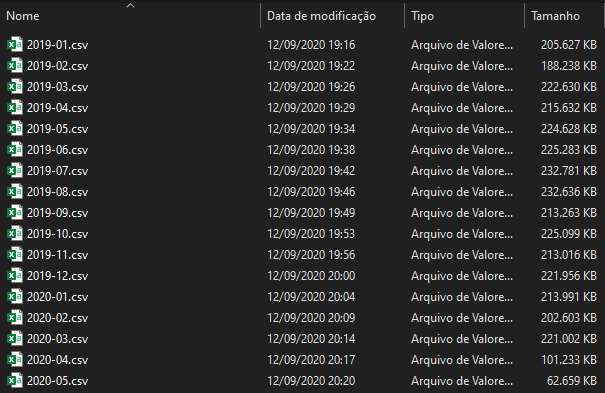
\includegraphics[scale = 0.5]{Imagens/Arquivos.png}
    \caption{Print dos arquivos}
    \label{fig: print}
\end{figure}

Já para a extração dos dados da FAA foi elaborado um script para fazer a busca e coleta dos dados das aeronaves utilizadas nos voos. Para fazer tal script também foi elaborado um arquivo .xlsx com todos os registros de aeronaves da BTS.

\subsection{Manipulação}




\section{Resultados}

Um primeiro resultado interessante já pôde ser observado na figura \ref{fig: print}. Lá pudemos ver, na última coluna, que o tamanho dos arquivos diminuiu muito nos meses de abril e maio de 2020 quando comparado aos demais meses, em especial no mesmo período de 2019, ou seja, os estadunidenses passaram a viajar menos e, com isso, o arquivo passou a ter menos dados. Isso já se mostrou ser um dos reflexos do coronavírus, uma vez que a população passou a ficar mais isolada.



\printbibliography

\end{document}
